\section{Preprocessing Techniques}\label{sec:preprocessing}
Understanding how to manipulate CSPs is necessary to gain an intuition for the limits of solving. There is not a universal theory for such things, but broad categories of techniques are useful to know about. This section will go through some of the most significant.

\subsection{Simplification}\label{sec:simplification}
Simplification is, intuitively, the first thing someone might want to do. Simplification will transform a CSP instance into another, smaller instance with the "same" solution.

These techniques are generally going to be highly specialized to the specific domain. Often, they will be limited to specific forms. For example, in boolean SAT, $x \vee x \vee y$ can be simplified into $x \vee y$. The most well-known simplification methods come from equational theories. Some methods are not immediately applicable due to CSPs splitting all their relations into clauses. For example, the simple factoring property, $(x-1) (x+1) = x^2 - 1$ does not immediately apply since the left and right sides will not generally represent atomic constraints. We may, instead, have the following available atomic constraints;

\begin{equation}
    a = C\ \text{for any constant}\ C
\end{equation}
\begin{equation}
    a = b + c
\end{equation}
\begin{equation}
    a = b \times c
\end{equation}

We may set up the left-hand-side of the factoring example as the following instance;

\begin{equation}
    o = 1 \wedge n = -1 \wedge a_1 = x + o \wedge a_2 = x + n \wedge m = a_1 \times a_2
\end{equation}

The factoring property would transform this into

\begin{equation}
    n = -1 \wedge s = x \times x \wedge m = s + n
\end{equation}

This is not a simplification according to a naive interpretation of the \say{same solution}. Notice that the variables are different, meaning a solution to this new problem would not actually be a solution to the old problem.

There is a certain sense that this problem is equivalent to the old one. The new problem is satisfiable if and only if the old one is. Further, the values of unshared variables can be uniquely determined by variables that are shared. As such, there is a 1-to-1 correspondence between solutions to the new instance and the old. More than that, the shared variables between the instances will share values within their satisfying assignments. This would allow one to easily calculate solutions to the old instance using solutions to the new instance. This defines a sense in which such transformed instances are \say{the same}.

Some previously mentioned techniques simplify problems. For example, fusing the boolean SAT clauses $x \vee y \vee \neg z$ and $z \vee w \vee v$ into $x \vee y \vee w \vee v$, using resolution as described in section \ref{sec:two-sat}, so long as $z$ is not mentioned in any other clause.

We can further use this idea to reason about our three-coloring example;

\begin{center}
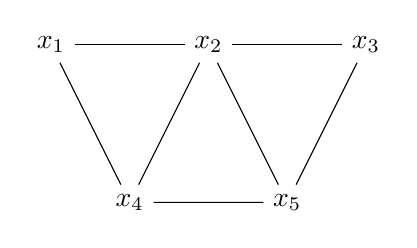
\begin{tikzpicture}
  \node (A) at (0,0) {$x_1$};
  \node (B) at (2,0) {$x_2$};
  \node (C) at (4,0) {$x_3$};
  \node (D) at (1,-2) {$x_4$};
  \node (E) at (3,-2) {$x_5$};

  \draw (A) -- (B) -- (C);
  \draw (A) -- (D) -- (E) -- (C);
  \draw (D) -- (B);
  \draw (E) -- (B);
\end{tikzpicture}
\end{center}

Given the naive interpretation of \say{the same} semantics, it seems like no simplification can be done. If we want to preserve semantics on the nose, then we must preserve nodes and can seemingly only change the edges. But, if we instead preserve semantics in the broader sense just described, we can make an immediate observation. The $x_1$ and $x_3$ nodes will have their color uniquely determined by the only two other nodes attached to them. This means we can eliminate them without changing the number of colorings. This gives us;

\begin{center}
\begin{tikzpicture}
  \node (B) at (2,0) {$x_2$};
  \node (D) at (1,-2) {$x_4$};
  \node (E) at (3,-2) {$x_5$};

  \draw (D) -- (E);
  \draw (D) -- (B);
  \draw (E) -- (B);
\end{tikzpicture}
\end{center}

We can further note that $x_2$ also has its color uniquely determined by the two nodes it is connected to. This, too, allows its elimination, leaving;

\begin{center}
\begin{tikzpicture}
  \node (D) at (1,-2) {$x_4$};
  \node (E) at (3,-2) {$x_5$};

  \draw (D) -- (E);
\end{tikzpicture}
\end{center}

This is now as simple as it can be. We can pick any pair of distinct colors for this pair, and it will determine a unique coloring for our original graph. This implies, in particular, that the number of colorings in our original graph is the same as the number of distinct color pairs; 6.

This idea can be nicely captured by string-diagram representations of CSP instances. In it, each relation becomes a node on a graph and each variable becomes a string connecting nodes. Variables mentioned by three or more relations get combined into "spider" nodes, represented by a lack of a node marker. This string diagram representation is a kind of duel of the other graph representation we have been using; swapping edges and nodes. The utility of this representation can be seen in the rewrite rule for our factoring example;

\begin{center}
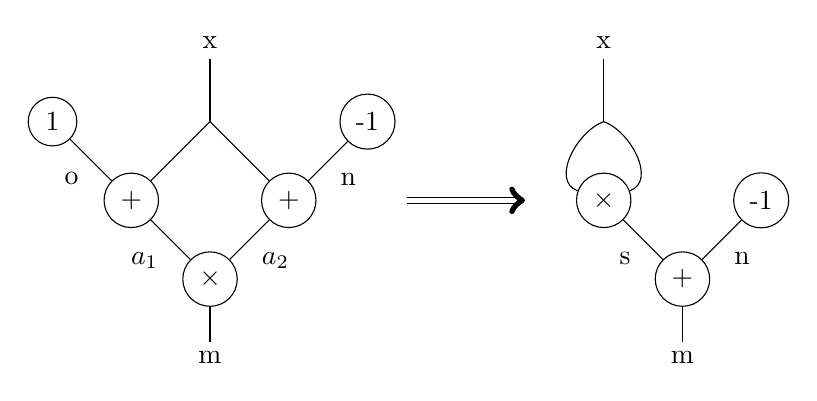
\begin{tikzpicture}[every label/.style={draw=none, text=black}]

    % Left string diagram
    % Nodes
    \node[] (x1) at (2,3) {x};
    \node[circle, draw] (1) at (0,2) {1};
    \node[circle, draw] (neg1) at (4,2) {-1};
    \node[coordinate] (coord1) at (2,2) {};
    \node[circle, draw] (+1) at (1,1) {+};
    \node[circle, draw] (+2) at (3,1) {+};
    \node[circle, draw] (times1) at (2,0) {$\times$};
    \node[] (m1) at (2,-1) {m};

    % Edges
    \draw (1) -- node[below left=1pt] {o} (+1);
    \draw (neg1) -- node[below right=1pt] {n} (+2);
    \draw (coord1) -- (+1);
    \draw (coord1) -- (+2);
    \draw (+1) -- node[below left=1pt] {$a_1$} (times1);
    \draw (+2) -- node[below right=1pt] {$a_2$} (times1);
    \draw (x1) -- (coord1);
    \draw (times1) -- (m1);

    % Right string diagram
    % Nodes
    \node[] (x2) at (7,3) {x};
    \node[coordinate] (coord2) at (7,2) {};
    \node[circle, draw] (times2) at (7,1) {$\times$};
    \node[circle, draw] (neg2) at (9,1) {-1};
    \node[circle, draw] (+3) at (8,0) {+};
    \node[] (m2) at (8,-1) {m};

    % Edges
    \draw (coord2) to[out=200,in=160] (times2);
    \draw (coord2) to[out=340,in=20] (times2);
    \draw (times2) -- node[below left=1pt] {s} (+3);
    \draw (neg2) -- node[below right=1pt] {n} (+3);
    \draw (x2) -- (coord2);
    \draw (+3) -- (m2);

    % Arrow between diagrams
    \draw[->, double distance between line centers=2pt] (4.5,1) -- (6,1);
\end{tikzpicture}
\end{center}

Drawing this rule using the ordinary graph representation would be difficult due to the many nodes an edge can have, but string diagrams handle such cases elegantly.

The string diagram for our recurring graph example would look like this;

\begin{center}
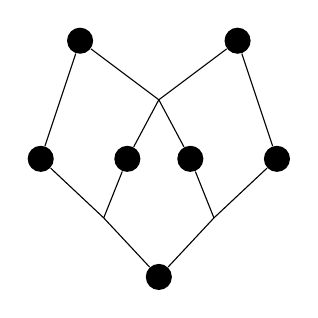
\begin{tikzpicture}
    % Row 1
    \node[fill=black, circle] (n1) at (0,0) {};
    \node[fill=black, circle] (n2) at (2,0) {};

    % Row 2
    \node[coordinate] (i1) at (1,-0.75) {};

    % Row 3
    \node[fill=black, circle] (n3) at (-0.5,-1.5) {};
    \node[fill=black, circle] (n4) at (0.6,-1.5) {};
    \node[fill=black, circle] (n5) at (1.4,-1.5) {};
    \node[fill=black, circle] (n6) at (2.5,-1.5) {};

    % Row 4
    \node[coordinate] (i2) at (0.3,-2.25) {};
    \node[coordinate] (i3) at (1.7,-2.25) {};

    % Row 5
    \node[fill=black, circle] (n7) at (1,-3) {};

    % Edges
    \draw (n1) -- (n3);
    \draw (n2) -- (n6);
    \draw (n1) -- (i1);
    \draw (n2) -- (i1);
    \draw (n4) -- (i1);
    \draw (n5) -- (i1);
    \draw (n3) -- (i2);
    \draw (n4) -- (i2);
    \draw (n7) -- (i2);
    \draw (n5) -- (i3);
    \draw (n6) -- (i3);
    \draw (n7) -- (i3);
\end{tikzpicture}
\end{center}

We can, further, draw the transformation rule eliminating nodes for graph coloring through the following rule;

\begin{center}
\begin{tikzpicture}[>=stealth]
    % Left Side
    % Top Node
    \node[coordinate] (topLeft) at (0,1.5) {};
    \draw (topLeft) -- ++(0.4, 0.4);
    \draw (topLeft) -- ++(-0.4, 0.4);
    \node[above=0.1cm of topLeft] {$\cdots$};
    
    % Middle Nodes
    \node[fill=black,circle] (midLeft1) at (0,1) {};
    \node[fill=black,circle, below=0.5cm of midLeft1] (midLeft2) {};
    \node[fill=black,circle, below right=0.25cm of midLeft1] (midLeft3) {};
    
    % Bottom Node
    \node[coordinate, below=0.5cm of midLeft2] (botLeft) {};
    \draw (botLeft) -- ++(0.4, -0.4);
    \draw (botLeft) -- ++(-0.4, -0.4);
    \node[below=0.1cm of botLeft] {$\cdots$};
    
    % Edges
    \draw (topLeft) -- (midLeft1) -- (midLeft2) -- (botLeft);
    \draw (topLeft) -- (midLeft3) -- (botLeft);
    
    % Right Side
    % Top Node
    \node[coordinate, right=4cm of topLeft] (topRight) {};
    \draw (topRight) -- ++(0.4, 0.4);
    \draw (topRight) -- ++(-0.4, 0.4);
    \node[above=0.1cm of topRight] {$\cdots$};

    \node[fill=black,circle, below=0.8cm of topRight] (topMid) {};
    
    % Bottom Node
    \node[coordinate, below=2cm of topRight] (botRight) {};
    \draw (botRight) -- ++(0.4, -0.4);
    \draw (botRight) -- ++(-0.4, -0.4);
    \node[below=0.1cm of botRight] {$\cdots$};
    
    \draw (topRight) -- (topMid) -- (botRight);
    
    % Double Arrow
    \draw[->, double] (1.8, 0.5) -- ++(0.5, 0);
\end{tikzpicture}
\end{center}

Repeatedly applying this to our string diagram, we would get the sequence;

\begin{center}
\begin{tikzpicture}
    % Row 1
    \node[fill=black, circle] (n1) at (0,0) {};
    \node[fill=black, circle] (n2) at (2,0) {};

    % Row 2
    \node[coordinate] (i1) at (1,-0.75) {};

    % Row 3
    \node[fill=black, circle] (n3) at (-0.5,-1.5) {};
    \node[fill=black, circle] (n4) at (0.6,-1.5) {};
    \node[fill=black, circle] (n5) at (1.4,-1.5) {};
    \node[fill=black, circle] (n6) at (2.5,-1.5) {};

    % Row 4
    \node[coordinate] (i2) at (0.3,-2.25) {};
    \node[coordinate] (i3) at (1.7,-2.25) {};

    % Row 5
    \node[fill=black, circle] (n7) at (1,-3) {};

    % Edges
    \draw (n1) -- (n3);
    \draw (n2) -- (n6);
    \draw (n1) -- (i1);
    \draw (n2) -- (i1);
    \draw (n4) -- (i1);
    \draw (n5) -- (i1);
    \draw (n3) -- (i2);
    \draw (n4) -- (i2);
    \draw (n7) -- (i2);
    \draw (n5) -- (i3);
    \draw (n6) -- (i3);
    \draw (n7) -- (i3);

    % Double Arrow
    \draw[->, double] (3.0, -1.5) -- ++(0.5, 0);



    % Row 1
    \node[right=3cm of n2, fill=black, circle] (n22) {};

    % Row 2
    \node[coordinate, right=4cm of i1] (i12) {};

    % Row 3
    \node[right=3cm of n4, fill=black, circle] (n42) {};
    \node[right=3cm of n5, fill=black, circle] (n52) {};
    \node[right=3cm of n6, fill=black, circle] (n62) {};

    % Row 4
    \node[coordinate, right=3cm of i3] (i32) {};

    % Row 5
    \node[right=3cm of n7, fill=black, circle] (n72) {};

    % Edges
    \draw (n22) -- (n62);
    \draw (n22) -- (i12);
    \draw (n42) -- (i12);
    \draw (n52) -- (i12);
    \draw (n42) -- (n72);
    \draw (n52) -- (i32);
    \draw (n62) -- (i32);
    \draw (n72) -- (i32);

    % Double Arrow
    \draw[->, double] (6.3, -1.5) -- ++(0.5, 0);



    % Row 3
    \node[right=3cm of n42, fill=black, circle] (n43) {};
    \node[right=3cm of n52, fill=black, circle] (n53) {};

    % Row 5
    \node[right=3cm of n72, fill=black, circle] (n73) {};

    % Edges
    \draw (n43) -- (n53);
    \draw (n43) -- (n73);
    \draw (n53) -- (n73);

    % Double Arrow
    \draw[->, double] (8.5, -1.5) -- ++(0.5, 0);



    % Row 3
    \node[right=2cm of n43] (n44) {};
    \node[right=2cm of n53] (n54) {};

    % Row 5
    \node[right=2cm of n73, fill=black, circle] (n74) {};

    % Edges
    \draw (n44) -- (n74);
    \draw (n54) -- (n74);
\end{tikzpicture}
\end{center}

Ending with a diagram equivalent to a single edge with two nodes in our previous representation. If we want to reconstruct a solution to the original CSP instance, we must also keep track of what rewrites we did, as those will correspond to functions calculating implied values for the original instance's variables.

This representation turns the simplification of a CSP into the actual simplification of a concrete data structure where the elimination of a variable becomes the elimination of an edge and the introduction of a variable corresponds to the introduction of an edge. Essentially all typical examples of algebraic simplification methods can be recast as local string-diagram rewrite rules. 

Tactics along these lines are studied widely within the subject of string diagrams. See \citep{bonchi2017functorial} for a broad account of relational theories presented as string diagrams. This also covers methods beyond simplification, such as strengthening instances to new ones which, if true, would imply a satisfying instance of the whole, but which are not equivalent. Such methods are important for implementing search, but will not be covered here. Some specific CSPs have fully worked out string diagram calculi that are algebraically complete; see \citep{gu2023complete} on boolean SAT, for example.

\subsection{Redundancy Elimination}\label{sec:redundancy}

The concepts from the previous section can be generalized to a notion of redundancy elimination. When solving a CSP, we care less about preserving the number of solutions than we do finding some solution. A transformation that preserves satisfiability, but not solution number, is fine for most purposes.

In general, we can ask if, given an instance $F \wedge C$, if removing $C$ preserves satisfiability. If so, then $C$ is redundant in the instance. This is all we need if we only care about the existence of a satisfying assignment. However, we generally actually want to find a solution. The most common method to reconstruct solutions through redundancy elimination are special cases of what is called \say{propagation redundancy}.

We can assess whether some clause is propagation redundant with respect to CSP instances by asking about assignments blocked by that clause. For example, if we have the clause $x = 1$, then the assignment $\langle x \rightarrow 0\rangle$ is blocked by that clause. As another example, the clause $\neg x \vee y \vee z$ blocks the assignment $\langle x \rightarrow 1, y \rightarrow 0, z \rightarrow 0\rangle$.

Given a partial assignment, $\alpha$, and a CSP instance, $F$, we denote the substitution of $\alpha$ info $F$ by $F_{|\alpha}$, creating the new, smaller CSP instance.

Given a clause, $C$, and a partial assignment, $\alpha$, blocked by that clause, we say that $C$ is propagation redundant with respect to the instance $F$ if there exists another partial assignment $\omega$ satisfying $C$, such that every assignment satisfying $F_{|\alpha}$ also satisfies $F_{|\omega}$, for every blocked assignment $\alpha$. We can frame this as the existence of a function, $f$, over partial assignments such that, for any blocked assignment, $\alpha$, any satisfying assignment for $F_{|\alpha}$ also satisfies $F_{|f(\alpha)}$.

The idea of this definition is that we have a CSP instance $F \wedge C$. Hypothetically, there is an assignment which we are looking for. It has a sub-assignment on the variables of $C$, $\alpha$, which may be blocked by $C$. That $C$ is redundant implies that we can replace if needed, the sub-assignment with another, $\omega$, which satisfies $C$ without causing $F$ to be unsatisfied. This means that given an assignment with sub-assignment $\alpha$ which satisfies $F$ but not $C$, an $\omega$ that we can swap with $\alpha$ will always exist so that $F \wedge C$ is satisfied in its entirety.

As a basic example, consider this 3-SAT problem;

\begin{equation}\label{equation:two-sat-example-pt1-2}
    (x \lor y) \land (x \lor z) \land (\neg x \lor y \lor z) \land x
\end{equation}

we may observe that $C = x$ blocks the assignment $\alpha = \langle x \rightarrow 0\rangle$. If we remove this clause, we would have.

\begin{equation}\label{equation:two-sat-example-pt1-2}
    F = (x \lor y) \land (x \lor z) \land (\neg x \lor y \lor z)
\end{equation}

We may also note that

\begin{equation}\label{equation:two-sat-example-pt1-2}
    F_{|\alpha} = y \land z
\end{equation}

We may observe that the only other partial assignment is $\omega = \langle x \rightarrow 1\rangle$, and

\begin{equation}\label{equation:two-sat-example-pt1-2}
    F_{|\omega} = y \lor z
\end{equation}

it is not hard to see that every satisfying assignment of $F_{|\alpha}$ also satisfies $F_{|\omega}$. If we have a satisfying assignment for $F$, there are two cases. Either it already also satisfies $F \wedge C$, in which case we are done, or it only satisfies $F$. As an example of the latter case, take the assignment $\langle x \rightarrow 0, y \rightarrow 1, z \rightarrow 1\rangle$. In the latter case, it must be a satisfying assignment of $F_{|\alpha}$. Since the sub-assignment $\langle y \rightarrow 1, z \rightarrow 1\rangle$ also satisfies $F_{|\omega}$, we can replace the $\alpha$ sub-assignment with $\omega$, getting $\langle x \rightarrow 1, y \rightarrow 1, z \rightarrow 1\rangle$ which satisfies $F \wedge C$.

As a second example, consider three coloring on the following graph;

\begin{center}
\begin{tikzpicture}
  \node (A) at (0,0) {$x_1$};
  \node (B) at (2,0) {$x_2$};
  \node (D) at (1,-2) {$x_4$};
  \node (E) at (3,-2) {$x_3$};

  \draw (A) -- (B);
  \draw (D) -- (E);
  \draw (D) -- (B);
  \draw (E) -- (B);
\end{tikzpicture}
\end{center}

This corresponds to the CSP instance;

\begin{equation}
    x_1 \neq x_2 \wedge x_2 \neq x_3 \wedge x_2 \neq x_4\wedge x_3 \neq x_4 
\end{equation}

It seems intuitively obvious that

\begin{equation}
    C = x_1 \neq x_2
\end{equation}

ought to be redundant as we should always be able to find an assignment satisfying it given an assignment for the rest;

\begin{equation}
    F = x_2 \neq x_3 \wedge x_2 \neq x_4\wedge x_3 \neq x_4 
\end{equation}

We may note that there are three assignments blocked by $C$. Without loss of generality, fix

\begin{equation}
    \alpha = \langle x_1 \rightarrow B, x_2 \rightarrow B\rangle
\end{equation}

We may note that;

\begin{equation}
    F_{|\alpha} = B \neq x_3 \neq x_4
\end{equation}

We may identify the following;

\begin{equation}
    \omega = \langle x_1 \rightarrow R, x_2 \rightarrow B\rangle
\end{equation}

and further, we may observe that $F_{|\alpha} = F_{|\omega}$, meaning that any assignment satisfying one will also satisfy the other. That $\omega$ will satisfy $F \wedge C$ and that analogous assignments will exist for all blocked clauses implies that $C$ is propagation redundant.

In theory, we only need to find one $\omega$ as an alternative to the blocked $\alpha$ and swap to it if needed. However, finding such can be nontrivial. In general, judging if a clause is propagation redundant is, itself, an NP-complete problem. As such, much work has been done to characterize clauses whose propagation redundancy is efficiently detectable. The most popular of these are the so-called \say{blocked clauses} and their variants. Alternatively, some recent methods, such as the so-called "satisfaction-driven clause learning" methodology, recursively call an SAT solver to detect redundancy.

There is a further generalization of redundancy. Instead of asking for every assignment of $F_{|\alpha}$ to satisfy $F_{|f(\alpha)}$, we may instead ask for a function, $f$, over partial assignments such that any assignment $\rho$ of $F_{|\alpha}$ is also an assignment of $F_{|f(\rho, \alpha)}$, and, of course, $f(\rho, \alpha)$ should satisfy the redundant clause $C$. This allows $\omega$ to vary based on what assignment for $F$ we found, and $f$ is exactly the method to reconstruct assignments for larger problems from smaller sub-problems. Using this, we can establish $x_3 \neq x_4$ as redundant in our previous example with 

\begin{equation}
  f(\rho, \alpha) = \langle x_3 \rightarrow \text{if}\ \rho(x_2) \in \{R, B\}\ \text{then}\ G\ \text{else}\ R, x_4 \rightarrow \text{if}\ \rho(x_2) \in \{R, G\}\ \text{then}\ B\ \text{else}\ R \rangle.    
\end{equation}

Note that $x_3 \neq x_4$ is not propagation redundant since, for example, the blocked assignment $\alpha = \langle x_3 \rightarrow B, x_4 \rightarrow B\rangle$ will produce

\begin{equation}
    F_{|\alpha} = x_1 \neq x_2 \wedge x_2 \neq B,
\end{equation}

and we will not be able to find an $\omega$ such that every assignment of $F_{\alpha}$ is also an assignment of $F_{\omega}$. If we try, for example, $\omega = \langle x_3 \rightarrow R, x_4 \rightarrow B\rangle$, then

\begin{equation}
    F_{|\omega} = x_1 \neq x_2 \wedge x_2 \neq R \neq B
\end{equation}

which is clearly more, not less, specific than $F_{|\alpha}$. Further, if we try $\omega = \langle x_3 \rightarrow R, x_4 \rightarrow G\rangle$, we would get

\begin{equation}
    F_{|\omega} = x_1 \neq x_2 \wedge x_2 \neq R \neq G
\end{equation}

which is not satisfied by $\langle x_1 \rightarrow R, x_2 \rightarrow G\rangle$, despite that being a satisfying assignment of $F_{|\alpha}$.

We may also turn redundancy notions into rewrite rules along the lines of those described in \ref{sec:simplification}.

For a modern treatment, see \citep{heule2017short} and \citep{barnett2021non}.

% \subsection{Equality Detection}\label{sec:equality-detection}
% TODO

% \subsection{Implication Graphs}\label{sec:vertex-splitting}
% TODO


% \subsection{Arc Consistency}\label{sec:arc-consistency}
% TODO

\subsection{Vertex Splitting}\label{sec:vertex-splitting}

Vertex splitting is a generic method to split up CSP problems when instances are almost disconnected. Consider a CSP problem of the form $F \wedge G$ where the two sub-instances, $F$ and $G$, share a single variable, $x$, in common. Rather than solving the problem as a whole, we can, instead, eliminate the shared variable. We can do this by instantiating the variable with each possible value. In the boolean case, this creates four sub-problems, $F_{|\langle x \rightarrow 0 \rangle}$, $F_{|\langle x \rightarrow 1 \rangle}$, $G_{|\langle x \rightarrow 0 \rangle}$, $G_{|\langle x \rightarrow 1 \rangle}$. Assuming $F$ and $G$ are roughly equal in size, the size of the problem doubles. However, due to the exponential worst-case complexity of CSP solving, we go from $O(2^m)$ to $O(4 \times 2^{\frac{m}{2}}) = O(2^{\frac{m}{2} + 2})$, where $m$ is the number of variables, which will generally be much, much faster.

We can generalize this by identifying vertex separators instead of individual vertices. One can identify a vertex separator of the instance graph which splits the problem into two problems only connected by the fact that they share the variables in the separator. We then fix the values of all the variables in the separator. Assuming there were $n$ variables in the separator, we now have $2^{n+1}$ sub-problems, each, roughly, half the size of the original problem. This means the new (total) work will be $O(2^{n + 1}  2^{\frac{m}{2}}) = O(2^{n + \frac{m}{2} + 1})$. Compared to the original work of $O(2^m)$, if $n$ is small, this could be a considerable asymptotic efficiency boost. However, random SAT problems can’t generally be efficiently decomposed like this since their minimal vertex separator will have roughly the same number of variables as $m/2$, meaning we’d be back to $~O(2^m)$ work and wouldn’t gain any advantage. Also, finding minimum vertex separators is, itself, an NP-hard problem, but decent approximation algorithms do exist. See \citep{amir2001solving}.

Vertex elimination can also be used to make a problem more tree-like. Take our recurring example graph as an example;

\begin{center}
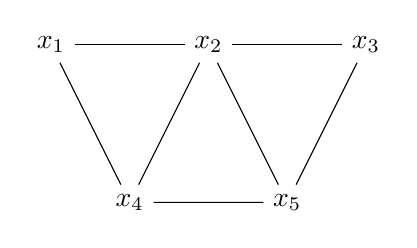
\begin{tikzpicture}
  \node (A) at (0,0) {$x_1$};
  \node (B) at (2,0) {$x_2$};
  \node (C) at (4,0) {$x_3$};
  \node (D) at (1,-2) {$x_4$};
  \node (E) at (3,-2) {$x_5$};

  \draw (A) -- (B) -- (C);
  \draw (A) -- (D) -- (E) -- (C);
  \draw (D) -- (B);
  \draw (E) -- (B);
\end{tikzpicture}
\end{center}

splitting $x_2$ would not split the problem, but it would make it entirely linear, allowing the sub-problems to be efficiently solved using the methods described in section \ref{sec:acyclic-queries}.

\subsection{Bound Variable Elimination}\label{sec:var-elim}

We can utilize the resolution method mentioned in section \ref{sec:two-sat} to eliminate variables in general. Restricted to the boolean SAT setting, if we want to eliminate a variable, $x$, we resolve all clauses where $x$ appears positively with every clause where it appears negatively. This creates the \say{clause distribution} of the variable. We then delete all the clauses mentioning $x$ and replace them with the clause distribution. As an example, consider the following;

\begin{equation}
    (x \vee y) \wedge (\neg y \vee z) \wedge (w \vee y) \wedge (\neg y \vee w)
\end{equation}

Let us eliminate $y$. Since $y$ appears in all these clauses, we will be replacing the whole instance. We can create the following table showing the clause distribution:

\begin{table}[h]
    \centering
    \begin{tabular}{c|c|c}
        & \( \neg y \vee z \) & \( \neg y \vee w \) \\
        \hline
        \( x \vee y \) & \( x \vee z \) & \( x \vee w \) \\
        \hline
        \( w \vee y \) & \( w \vee z \) & \( w \) \\
    \end{tabular}
    \label{tab:clause-distribution}
\end{table}

After eliminating \(y\), the new instance becomes:
\begin{equation}
(x \vee z) \wedge (x \vee w) \wedge (w \vee z) \wedge (w)
\end{equation}

Finding an assignment, at this point, becomes a trivial exercise. Given an assignment for the new instance, we can derive an assignment for $y$ by applying that assignment to the positive clauses for $y$, along with assigning $y$ to be false. If any of them are false, then $y$ must be true, otherwise, it may be false in a full assignment. This choice is somewhat arbitrary; we could have applied the assignment to the negative clauses for $y$, along with assigning $y$ to be true, getting a similar analysis.

Two special cases are important to note. Firstly, if a variable only appears as positive or negative, then the clause distribution will be empty. This reflects the fact that we may eliminate such a variable by assigning it a value that satisfies all the clauses it appears in. Secondly, if the variable appears in a singleton/unit clause, then the distribution will be logically equivalent to either the positive or negative clauses with the variable removed. This reflects the fact that unit clauses force a value for their variable.

If we take a step back, we can understand what resolution is doing. We may restate the resolution as stating;

\begin{equation}\label{equation:binary-resolution-2}
\frac{p = 0 \rightarrow C_1 \quad p = 1 \rightarrow C_2}{C_1 \lor C_2}
\end{equation}

In the boolean case, we have full coverage with the two cases. In the case of three-valued CSPs, we may have more complex resolution variants;

\begin{align}
\frac{p = 0 \rightarrow C_1 \quad p = 1 \rightarrow C_2 \quad p = 2 \rightarrow C_2}{C_1 \lor C_2 \lor C_3} \quad
\frac{(p = 0 \vee p = 1) \rightarrow C_1 \quad p = 2 \rightarrow C_2}{C_1 \lor C_2} \nonumber \\
\frac{(p = 0 \vee p = 2) \rightarrow C_1 \quad p = 1 \rightarrow C_2}{C_1 \lor C_2} \quad
\frac{(p = 1 \vee p = 2) \rightarrow C_1 \quad p = 0 \rightarrow C_2}{C_1 \lor C_2} \label{equation:binary-resolution-3-all}
\end{align}

We may even extend this into the infinite domain. If our domain is the integers, then the following is a valid resolution variant;

\begin{equation}\label{equation:binary-resolution-Z}
\frac{p < 0 \rightarrow C_1 \quad p \geq 0 \rightarrow C_2}{C_1 \lor C_2}
\end{equation}

Though it becomes more complicated as the domain grows, there is a natural extension of clause distribution. Applicability will depend on the extent we may interpret a clause as an implication of the appropriate form. If we take three-coloring as an example, we only have one kind of clause, of the form $x \neq y$. We can rephrase this as;

\begin{align}
    (x = R) &\rightarrow (y = G \vee y = B)\ \wedge \nonumber \\
    (x = G) &\rightarrow (y = R \vee y = B)\ \wedge \nonumber \\
    (x = B) &\rightarrow (y = R \vee y = G)\label{eq:multiline}
\end{align}

This will expand the formula, but put every clause in a form that is resolution compatible. Similarly, there is a form that places $y$ in the antecedent. Using this form, we may eliminate a variable, although we will be switching to a more flexible CSP since our clause distribution will not exclusively contain clauses of the form $x \neq y$.

\subsection{Cost Preservation}\label{sec:cost-preservation}

We have talked mostly about satisfaction, but, for the purposes of optimization, additional steps must be taken to ensure costs are preserved by transformations. Consider the following problem;

\begin{equation}
    (x \vee y) \wedge (\neg y \vee z) \wedge (w \vee y) \wedge (\neg y \vee w) \wedge (\neg x \vee \neg w) \wedge \neg w
\end{equation}

Assume our goal is to maximize the number of satisfied clauses. A maximum can be reached by assigning $\langle x \rightarrow 0, y \rightarrow 1, z \rightarrow 1, w \rightarrow 0 \rangle$, which satisfies 5 clauses, but this is not the only assignment that does this. 

it is entirely possible to eliminate all the variables using bound variable elimination. This will merely tell us that the statement is unsatisfiable.

If we used unit propagation to eliminate $w$, we would get

\begin{equation}
    (x \vee y) \wedge (\neg y \vee z) \wedge y \wedge \neg y
\end{equation}

This is also not satisfiable. The assignment $\langle x \rightarrow 1, y \rightarrow 0, z \rightarrow 1 \rangle$ satisfies 3 clauses, which is the max, though this is not the only way to do this. Unfortunately, this does not tell us anything about the maximum satisfiability of the original problem. If we reconstruct an assignment for the full problem from this by assigning $\langle w \rightarrow 0 \rangle$ (since the original unit clause negated $w$), we would only satisfy 4 of the original clauses, which is suboptimal.

How do we fix this?

The short answer is that we must introduce new variables whose value is directly tied to the value we seek to maximize, and we must ensure that these are not targeted for elimination. We start by adding a unique labeling variable to each clause;

\begin{equation}
    (x \vee y \vee l_1) \wedge (\neg y \vee z \vee l_2) \wedge (w \vee y \vee l_3) \wedge (\neg y \vee w \vee l_4) \wedge (\neg x \vee \neg w \vee l_5) \wedge (\neg w \vee l_6)
\end{equation}

We can now reframe our utility function as the sum of the negation of these labels. This new instance can be trivially satisfied by assigning them all true; we want to minimize the number we have to set to true.

We can start eliminating variables, ensuring that our labels remain untouched. First, eliminate $w$, getting;

\begin{equation}
    (x \vee y \vee l_1) \wedge (\neg y \vee z \vee l_2) \wedge (\neg x\lor y\lor l_3\lor l_5)\land (y\lor l_3\lor l_6)\land (\neg x\lor \neg y\lor l_4\lor l_5)\land (\neg y\lor l_4\lor l_6)
\end{equation}

We can then eliminate $x$, getting

\begin{equation}
(\neg y\lor z\lor l_2)\land (y\lor l_1\lor y\lor l_3\lor l_5)\land (y\lor l_3\lor l_6)\land (y\lor l_1\lor \neg y\lor l_4\lor l_5)\land (\neg y\lor l_4\lor l_6)
\end{equation}

We can remove the fourth of these clauses, since it is trivial, and simplify the second to get;

\begin{equation}
(\neg y\lor z\lor l_2)\land (y\lor l_1 \lor l_3\lor l_5)\land (y\lor l_3\lor l_6) \land (\neg y\lor l_4\lor l_6)
\end{equation}

We can eliminate $z$, getting;

\begin{equation}
(y\lor l_1 \lor l_3\lor l_5)\land (y\lor l_3\lor l_6) \land (\neg y\lor l_4\lor l_6)
\end{equation}

Incidentally, this eliminates the label $l_2$, which we can assign false since its covered by $z$. This tells us that allowing the second clause to be false cannot possibly help us find a maximizing assignment. Lastly, we can eliminate $y$, getting

\begin{equation}
    (l_4 \lor l_6\lor l_1\lor l_3\lor l_5)\land (l_4\lor l_6\lor l_3\lor l_6)
\end{equation}

and this can be cleaned up into;

\begin{equation}
    (l_1 \lor l_3\lor l_4\lor l_5\lor l_6)\land (l_3 \lor l_4\lor l_6)
\end{equation}

We may also notice that the second clause is more specific than the first, meaning we can drop the first clause without changing semantics (this is called \say{clause subsumption}), also eliminating $l_1$ and $l_5$ in the process. This gets;

\begin{equation}
    l_3 \lor l_4\lor l_6
\end{equation}

This gives us a full characterization of what we need to maximize satisfiability. We must have one of the clauses labeled by one of these to be false. If we, for example, choose $l_4$ to be the failing clause, then we are forced to assign $\langle y \rightarrow 1, w \rightarrow 0\rangle$, since that is the only assignment blocked by our fourth clause, $\neg y \vee w$. Removing this clause and substituting the blocked assignment, we would get a formula that must be satisfiable. In this case, we would get;

\begin{equation}
    z
\end{equation}

Which forces $z$ to be true, and allows $x$ to be anything. Any of these assignments will maximize satisfiability, and we can characterize all the other maximizing assignments by looking at the $l_3$ and $l_6$ branches.

See \citep{belov2013sat} and follow-up work for more information on this method.

\subsection{Decomposition in Integer Linear Programming}\label{sec:ilp-blocks}

The most popular method for solving integer programming problems involves decomposing the problem into a smaller problem. There are many ways to do this; this section will focus on the "branch and bound" method since it is the most popular.

Consider the following problem;

Maximize $5x_1 + 8x_2$ subject to the constraints $2x_1 + 3x_2 \leq 5$ and $4x_1 + 9x_2 \leq 12$. Our ultimate goal is to split up the problem into two easier sub-problems while removing regions guaranteed to not contain the optimum.

We may start by solving the relaxed problem. This means we solve the problem assuming $x_1$ and $x_2$ are rationals instead of integers. This will not generally give us an integer solution, but we can use it as an approximation that can be leveraged later on, and it can be found much more efficiently using non-integer linear programming methods. In this case, a maximum of $\frac{77}{6}$ is reached when $x_1 = \frac{3}{2}$ and $x_2 = \frac{2}{3}$.

From here, we create two new sub-problems by cutting on integer approximations of this solution. In this case, we will round $x_1$ up to $2$ in one problem, and down to $1$ in the other. This creates two sub-problems;

\begin{equation}
    x_1 \leq 1 \wedge 2x_1 + 3x_2 \leq 5 \wedge 4x_1 + 9x_2 \leq 12
\end{equation}

and 

\begin{equation}
    x_1 \geq 2 \wedge 2x_1 + 3x_2 \leq 5 \wedge 4x_1 + 9x_2 \leq 12
\end{equation}

One of these smaller regions is guaranteed to have the true, integer maximum. If we solve the relaxed version of these problems, we get the maximum at $x_1 = 1$ and $x_2 = \frac{8}{9}$ for the first problem, and at $x_1 = 2$ and $x_2 = \frac{1}{3}$ for the second. $x_2$ is not an integer for either of these, so we can cut on it, creating four sub-problems. In this case, the cut on both sub-problems will approximate $x_2$ down to $0$ and up to $1$, but, in general, cutting the same variable on different sub-problems will produce different approximations. In this case, our sub-problems are;

\begin{equation}
    x_1 \leq 1 \wedge x_2 = 0 \wedge 2x_1 + 3x_2 \leq 5 \wedge 4x_1 + 9x_2 \leq 12
\end{equation}

\begin{equation}
    x_1 \leq 1 \wedge x_2 \geq 1 \wedge 2x_1 + 3x_2 \leq 5 \wedge 4x_1 + 9x_2 \leq 12
\end{equation}

\begin{equation}
    x_1 \geq 2 \wedge x_2 = 0 \wedge 2x_1 + 3x_2 \leq 5 \wedge 4x_1 + 9x_2 \leq 12
\end{equation}

\begin{equation}
    x_1 \geq 2 \wedge x_2 \geq 1 \wedge 2x_1 + 3x_2 \leq 5 \wedge 4x_1 + 9x_2 \leq 12
\end{equation}

As it turns out, the last of these problems is unsatisfiable, so we throw it away. The first of these problems reaches its relaxed max at $x_1 = 1$ and $x_2 = 0$, with a max value of $5$. Since the relaxed max is an integer solution, this is also the max when restricted to integers. This is not necessarily the global max, but we will mark it down as the best possible solution found so far.

The other two problems reach a max at $x_1 = \frac{3}{4}$ and $x_2 = 0$ and $x_1 = \frac{5}{2}$ and $x_2 = 1$, respectively. These have a max value of $\frac{47}{4}$ and $\frac{25}{2}$, respectively. If either of these were less than $5$, we could eliminate them since they could not possibly have better integer solutions than what we have found so far, however, both are larger so we must continue. Integer approximating values of $x_1$ produces the four sub-problems;

\begin{equation}
    x_1 = 0 \wedge x_2 \geq 1 \wedge 2x_1 + 3x_2 \leq 5 \wedge 4x_1 + 9x_2 \leq 12
\end{equation}

\begin{equation}
    x_1 = 1 \wedge x_2 \geq 1 \wedge 2x_1 + 3x_2 \leq 5 \wedge 4x_1 + 9x_2 \leq 12
\end{equation}

\begin{equation}
    x_1 \geq 3 \wedge x_2 = 0 \wedge 2x_1 + 3x_2 \leq 5 \wedge 4x_1 + 9x_2 \leq 12
\end{equation}

\begin{equation}
    x_1 = 2 \wedge x_2 = 0 \wedge 2x_1 + 3x_2 \leq 5 \wedge 4x_1 + 9x_2 \leq 12
\end{equation}

The middle two problems are unsatisfiable, so we throw them away. The last problem has a relaxed integer solution at $x_1 = 2$ and $x_2 = 0$, with a value of 10; so that is our new best found so far. That first problem reaches a relaxed max at $x_1 = 0$ and $x_2 = \frac{4}{3}$. Its max value is $\frac{32}{3}$, which is more than $10$, so we continue. We cut on that first problem to get two sub-problems;

\begin{equation}
    x_1 = 0 \wedge x_2 = 1 \wedge 2x_1 + 3x_2 \leq 5 \wedge 4x_1 + 9x_2 \leq 12
\end{equation}

\begin{equation}
    x_1 = 0 \wedge x_2 \geq 2 \wedge 2x_1 + 3x_2 \leq 5 \wedge 4x_1 + 9x_2 \leq 12
\end{equation}

The second problem is unsatisfiable, while the first has a relaxed integer solution at $x_1 = 0$ and $x_2 = 1$, with a max value of $8$. This is the final sub-problem, so we know that our previous integer solution with a value of $10$ is, indeed, the maximum value possible.

This is just one decomposition method. There are myriad more ways to perform cuts and to decompose integer linear programming problems. See \citep{galati2010decomposition} for a modern overview.

\subsection{Other Methods}\label{sec:other-preproc}

There are numerous other preprocessing methods, far too many to cover here. A notable missing method is that of implication graphs, used for equality detection and clause learning. For a thorough treatment of techniques in the context of boolean SAT, see chapter 9 of \citep{biere2009handbook}.